\documentclass{beamer}
\usepackage{amsmath}
\usepackage{amssymb}
\usepackage{graphicx}
\usepackage{xcolor}
\usepackage{listings}
\usepackage{algorithm}
\usepackage{algpseudocode}
\usepackage{tikz}
\usepackage{empheq}


% Theme configuration
\usetheme{Madrid}
\usecolortheme{default}
\setbeamertemplate{navigation symbols}{}
\setbeamertemplate{footline}[frame number]

 
\begin{document}
\begin{frame}{Adding point-like sinks and sources}
    \vspace{-0.5cm}
    \onslide<1->{
        \begin{align*}
            \frac{\partial u}{\partial t} &= 
            D\Biggl( \frac{\partial^2 u}{\partial x^2} + \frac{\partial^2 u}{\partial y^2} \Biggr) 
            + K_{out} \sum_{p=1}^{N} \delta(r_p - r)
            - K_{in} \sum_{c=1}^{N} \delta(r_c - r)
        \end{align*}
    }
    \onslide<2->{
        We can discretize the first half-step ($x$ implicit, $y$ explicit) using the following scheme:

        \vspace{0.5cm}
             {\small % Optionally reduce font size
        \begin{equation*}
            \frac{u_{i,j}^{k+\frac{1}{2}} - u_{i,j}^{k}}{\Delta t/2}
            = D\Biggl(
            \frac{u_{i+1,j}^{k+\frac{1}{2}} - 2u_{i,j}^{k+\frac{1}{2}} + u_{i-1,j}^{k+\frac{1}{2}}}{\Delta x^2} + \frac{u_{i,j+1}^{k} - 2u_{i,j}^{k} + u_{i,j-1}^{k}}{\Delta y^2}
            \Biggr)
            + (S_{out} - S_{in})
        \end{equation*}
        }
       Where $S_{out}$ and $S_{in}$ are the source and sink terms, respectively:
        \begin{align*}
            S_{out} = K_{out} \sum_{p=1}^{N} \delta_{\varepsilon}(r_p - r_{i,j}) \quad \text{and} \quad
            S_{in} =  \frac{K_{in} u_{i,j}^{k}}{m + u_{i,j}^{k}} \sum_{c=1}^{N} \delta_{\varepsilon}(r_c - r_{i,j})
        \end{align*}
        }
    
\end{frame}

\begin{frame}
    \vspace{0.0cm}
    We can define $\alpha = \frac{D \Delta t}{2 \Delta x^2} = \frac{D \Delta t}{2 \Delta y^2}$ to get
    \begin{align*}
        \resizebox{\textwidth}{!}{%
$\boxed{\small 
\colorbox{red!20}{$ -\alpha u_{i-1,j}^{k+\frac{1}{2}} + (1 + 2\alpha)u_{i,j}^{k+\frac{1}{2}} - 
\alpha u_{i+1,j}^{k+\frac{1}{2}} $}= 
\colorbox{blue!20}{$\alpha u_{i,j-1}^k + (1 - 2\alpha)u_{i,j}^k + \alpha u_{i,j+1}^k
+ 
\frac{\Delta t}{2} \left(S_{out} - S_{in}
\right)$}}$}
\end{align*}
    We know all the terms in right-hand side of the equation (blue), but we need to compute the left-hand side (red). 
\end{frame}




\begin{frame}{Writing the tridiagonal matrix}
    \vspace{-0.8cm}   
    Let's fix $j = 1$ and write the equations for $i =  1, 2, 3, 4$:
    
    \begin{columns}
        \begin{column}{0.3\textwidth}
            % Place both figures in a row here
            \begin{minipage}{0.2\textwidth}
                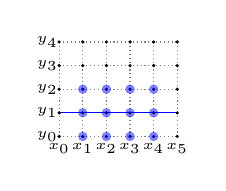
\begin{tikzpicture}[scale=0.3]
                    \foreach \y in {0,...,4} {
                         \draw[gray, densely dotted] (0,\y) -- (5,\y);
                         \node at (-0.5, \y) {\tiny$y_{\y}$};
                         \ifnum \y = 1
                            \draw[blue, thin] (0,1) -- (5,1);
                         \fi
                     }
                                         
                     \foreach \x in {0,...,5} {
                         \draw[gray, densely dotted] (\x,0) -- (\x,4);
                         \node at (\x, -0.5) {\tiny$x_{\x}$};
                     }
                     \foreach \x in {0,...,5}
                         \foreach \y in {0,...,4} {
                             \fill (\x,\y) circle (0.0753);
                             \onslide<3->{  
                             \ifnum \x=1 \ifnum \y=0
                                 \fill[blue, fill opacity=0.5] (\x,\y) circle (0.2);
                             \fi \fi
                             \ifnum \x=1\ifnum \y=1
                                 \fill[blue, fill opacity=0.5] (\x,\y) circle (0.2);
                             \fi \fi
                             \ifnum \x=1 \ifnum \y=2
                                 \fill[blue, fill opacity=0.5] (\x,\y) circle (0.2);
                             \fi \fi
                             }
                            \onslide<4->{
                                \ifnum \x=2 \ifnum \y=0
                                    \fill[blue, fill opacity=0.5] (\x,\y) circle (0.2);
                                \fi \fi
                                \ifnum \x=2\ifnum \y=1
                                    \fill[blue, fill opacity=0.5] (\x,\y) circle (0.2);
                                \fi \fi
                                \ifnum \x=2 \ifnum \y=2
                                    \fill[blue, fill opacity=0.5] (\x,\y) circle (0.2);
                                \fi \fi
                                }
                            \onslide<5->{
                                \ifnum \x=3 \ifnum \y=0
                                    \fill[blue, fill opacity=0.5] (\x,\y) circle (0.2);
                                \fi \fi
                                \ifnum \x=3\ifnum \y=1
                                    \fill[blue, fill opacity=0.5] (\x,\y) circle (0.2);
                                \fi \fi
                                \ifnum \x=3 \ifnum \y=2
                                    \fill[blue, fill opacity=0.5] (\x,\y) circle (0.2);
                                \fi \fi
                                }
                            \onslide<6->{
                                \ifnum \x=4 \ifnum \y=0
                                    \fill[blue, fill opacity=0.5] (\x,\y) circle (0.2);
                                \fi \fi
                                \ifnum \x=4\ifnum \y=1
                                    \fill[blue, fill opacity=0.5] (\x,\y) circle (0.2);
                                \fi \fi
                                \ifnum \x=4 \ifnum \y=2
                                    \fill[blue, fill opacity=0.5] (\x,\y) circle (0.2);
                                \fi \fi
                                }

                         }
                         
                 \end{tikzpicture}
                \end{minipage}\\
            \vspace{-0.2cm}
            \onslide<2->{
            \begin{center}
               
            \end{center}
            \vspace{-0.2cm}
            \begin{minipage}{0.3\textwidth}
                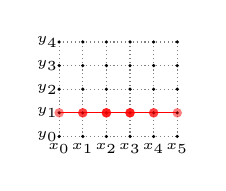
\begin{tikzpicture}[scale=0.3]
                    \foreach \y in {0,...,4} {
                         \draw[gray, densely dotted] (0,\y) -- (5,\y);
                         \node at (-0.5, \y) {\tiny$y_{\y}$};
                         \ifnum \y = 1
                         \draw[red, thin] (0,1) -- (5,1);
                      \fi
                     }
                                         
                     \foreach \x in {0,...,5} {
                         \draw[gray, densely dotted] (\x,0) -- (\x,4);
                         \node at (\x, -0.5) {\tiny$x_{\x}$};
                     }
                     \foreach \x in {0,...,5}
                         \foreach \y in {0,...,4} {
                             \fill (\x,\y) circle (0.0753);
                            \onslide<3->{
                             \ifnum \x=0 \ifnum \y=1
                                 \fill[red, fill opacity=0.5] (\x,\y) circle (0.2);
                             \fi \fi
                             \ifnum \x=1\ifnum \y=1
                                 \fill[red, fill opacity=0.5] (\x,\y) circle (0.2);
                             \fi \fi
                             \ifnum \x=2 \ifnum \y=1
                                 \fill[red, fill opacity=0.5] (\x,\y) circle (0.2);
                             \fi \fi
                         }
                         \onslide<4->{
                             \ifnum \x=1 \ifnum \y=1
                                 \fill[red, fill opacity=0.5] (\x,\y) circle (0.2);
                             \fi \fi
                             \ifnum \x=2\ifnum \y=1
                                 \fill[red, fill opacity=0.5] (\x,\y) circle (0.2);
                             \fi \fi
                             \ifnum \x=3 \ifnum \y=1
                                 \fill[red, fill opacity=0.5] (\x,\y) circle (0.2);
                             \fi \fi
                         }
                            \onslide<5->{
                                \ifnum \x=2 \ifnum \y=1
                                    \fill[red, fill opacity=0.5] (\x,\y) circle (0.2);
                                \fi \fi
                                \ifnum \x=3\ifnum \y=1
                                    \fill[red, fill opacity=0.5] (\x,\y) circle (0.2);
                                \fi \fi
                                \ifnum \x=4 \ifnum \y=1
                                    \fill[red, fill opacity=0.5] (\x,\y) circle (0.2);
                                \fi \fi
                            }
                            \onslide<6->{
                                \ifnum \x=3 \ifnum \y=1
                                    \fill[red, fill opacity=0.5] (\x,\y) circle (0.2);
                                \fi \fi
                                \ifnum \x=4\ifnum \y=1
                                    \fill[red, fill opacity=0.5] (\x,\y) circle (0.2);
                                \fi \fi
                                \ifnum \x=5 \ifnum \y=1
                                    \fill[red, fill opacity=0.5] (\x,\y) circle (0.2);
                                \fi \fi
                            }
                         
                         }
                \end{tikzpicture}
            \end{minipage}
            }
        \end{column}
        \hspace{-1.5cm}
       \begin{column}{0.7\textwidth}
            \footnotesize
            
            \vspace{-0.6cm}
            
            \onslide<3->{
                {\tiny
                \begin{align*}
                    -\alpha \textcolor{red}{u_{0,j}^{k+\frac{1}{2}}} + (1 + 2\alpha)\textcolor{red}{u_{1,j}^{k+\frac{1}{2}}}
                    - \alpha \textcolor{red}{u_{2,j}^{k+\frac{1}{2}}}
                    = \alpha \textcolor{blue}{u_{1,j-1}^k} + (1 - 2\alpha)\textcolor{blue}{u_{1,j}^k} + \alpha \textcolor{blue}{u_{1,j+1}^k} + 
                     \frac{\Delta t}{2} \left(S_{out} - S_{in}\right)
                \end{align*}
                }
            }
            \vspace{-0.611cm}
            \onslide<4->{
                {\tiny
                \begin{align*}
                    -\alpha \textcolor{red}{u_{1,j}^{k+\frac{1}{2}}} + (1 + 2\alpha)\textcolor{red}{u_{2,j}^{k+\frac{1}{2}}}
                    - \alpha \textcolor{red}{u_{3,j}^{k+\frac{1}{2}}}
                    = \alpha \textcolor{blue}{u_{2,j-1}^k} + (1 - 2\alpha)\textcolor{blue}{u_{2,j}^k} + \alpha \textcolor{blue}{u_{2,j+1}^k} + 
                    \frac{\Delta t}{2} \left(S_{out} - S_{in}\right)
                \end{align*}
                }
            }
            \vspace{-0.611cm}
            \onslide<5->{
                {\tiny
                \begin{align*}
                    -\alpha \textcolor{red}{u_{2,j}^{k+\frac{1}{2}}} + (1 + 2\alpha)\textcolor{red}{u_{3,j}^{k+\frac{1}{2}}}
                    - \alpha \textcolor{red}{u_{4,j}^{k+\frac{1}{2}}}
                    = \alpha \textcolor{blue}{u_{3,j-1}^k} + (1 - 2\alpha)\textcolor{blue}{u_{3,j}^k} + \alpha \textcolor{blue}{u_{3,j+1}^k} + 
                    \frac{\Delta t}{2} \left(S_{out} - S_{in}\right)
                \end{align*}
                }
            }
            \vspace{-0.611cm}
            \onslide<6->{
                {\tiny
                \begin{align*}
                    -\alpha \textcolor{red}{u_{3,j}^{k+\frac{1}{2}}} + (1 + 2\alpha)\textcolor{red}{u_{4,j}^{k+\frac{1}{2}}}
                    - \alpha \textcolor{red}{u_{5,j}^{k+\frac{1}{2}}}
                    = \alpha \textcolor{blue}{u_{4,j-1}^k} + (1 - 2\alpha)\textcolor{blue}{u_{4,j}^k} + \alpha \textcolor{blue}{u_{4,j+1}^k} +
                    \frac{\Delta t}{2} \left(S_{out} - S_{in}\right)
                \end{align*}
                }
            }
            \vspace{-0.5cm}
            \onslide<7->{
            Which can be written as a matrix:
            }
            \vspace{-0.3cm}
            \onslide<8->{
                \begin{align*}
                    \begin{bmatrix}
                        -\alpha & 1 + 2\alpha & -\alpha & 0 & 0 & 0 \\
                        0 & -\alpha & 1 + 2\alpha & -\alpha & 0 & 0 \\
                        0 & 0 & -\alpha & 1 + 2\alpha & -\alpha & 0 \\
                        0 & 0 & 0 & -\alpha & 1 + 2\alpha & -\alpha \\
                    \end{bmatrix}
                    \begin{bmatrix}
                        \textcolor{red}{u_{0,j}^{k+\frac{1}{2}}} \\
                        \textcolor{red}{u_{1,j}^{k+\frac{1}{2}}} \\
                        \textcolor{red}{u_{2,j}^{k+\frac{1}{2}}} \\
                        \textcolor{red}{u_{3,j}^{k+\frac{1}{2}}} \\
                        \textcolor{red}{u_{4,j}^{k+\frac{1}{2}}} \\
                        \textcolor{red}{u_{5,j}^{k+\frac{1}{2}}}
                    \end{bmatrix}
                    =
                    \begin{bmatrix}
                        \textcolor{blue}{b_{1,j}} \\
                        \textcolor{blue}{b_{2,j}} \\
                        \textcolor{blue}{b_{3,j}} \\
                        \textcolor{blue}{b_{4,j}} \\
                    \end{bmatrix}
                \end{align*}
            Where $\textcolor{blue}{b_{i,j}}$ is the right hand side of the equation, which is already known.
            }
        \end{column}
    \end{columns}
\onslide<9->{
    \small
    Because of the boundary conditions, we can simplify the matrix to a tridiagonal matrix.
}
    \vspace{-1cm}
\end{frame}


\begin{frame}{Writing the tridiagonal matrix}
    \vspace{-0.8cm}   
    We get one system of equations for each $j$ value.
    
    \begin{columns}
        \begin{column}{0.3\textwidth}
            % Place both figures in a row here
            \begin{minipage}{0.48\textwidth}
                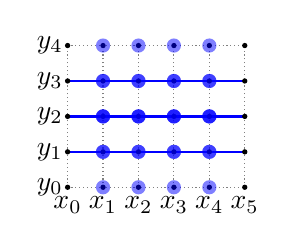
\begin{tikzpicture}[scale=0.45]
                    \foreach \y in {0,...,4} {
                         \draw[gray, densely dotted] (0,\y) -- (5,\y);
                         \node at (-0.5, \y) {$y_{\y}$};
                         \onslide<2->{
                         \ifnum \y = 1
                         \draw[blue, thick] (0,1) -- (5,1);
                      \fi
                         }
                         \onslide<3->{
                            \ifnum \y = 2
                            \draw[blue, thick] (0,2) -- (5,2);
                            \fi
                         }
                         \onslide<4->{
                            \ifnum \y = 3
                            \draw[blue, thick] (0,3) -- (5,3);
                            \fi
                         }
                     } 
                                         
                     \foreach \x in {0,...,5} {
                         \draw[gray, densely dotted] (\x,0) -- (\x,4);
                         \node at (\x, -0.5) {$x_{\x}$};
                     }
                     \foreach \x in {0,...,5}
                         \foreach \y in {0,...,4} {
                             \fill (\x,\y) circle (0.0753); 
                             \onslide<2->{
                             \ifnum  \y=1 \ifnum  \x>0 \ifnum  \x<5
                                 \fill[blue, fill opacity=0.5] (\x,\y) circle (0.2);
                            \fi \fi \fi
                            \ifnum  \y=2  \ifnum  \x>0 \ifnum  \x<5
                                \fill[blue, fill opacity=0.5] (\x,\y) circle (0.2);
                                \fi \fi \fi
                            \ifnum  \y=0 \ifnum  \x>0 \ifnum  \x<5
                                \fill[blue, fill opacity=0.5] (\x,\y) circle (0.2);
                                \fi \fi \fi 
                             }
                             \onslide<3->{
                                \ifnum  \y=1 \ifnum  \x>0 \ifnum  \x<5
                                    \fill[blue, fill opacity=0.5] (\x,\y) circle (0.2);
                                \fi \fi \fi
                                \ifnum  \y=2  \ifnum  \x>0 \ifnum  \x<5
                                    \fill[blue, fill opacity=0.5] (\x,\y) circle (0.2);
                                    \fi \fi \fi
                                \ifnum  \y=3 \ifnum  \x>0 \ifnum  \x<5
                                    \fill[blue, fill opacity=0.5] (\x,\y) circle (0.2);
                                    \fi \fi \fi 
                                 }
                           \onslide<4->{
                                \ifnum  \y=2 \ifnum  \x>0 \ifnum  \x<5
                                    \fill[blue, fill opacity=0.5] (\x,\y) circle (0.2);
                                \fi \fi \fi
                                \ifnum  \y=3  \ifnum  \x>0 \ifnum  \x<5
                                    \fill[blue, fill opacity=0.5] (\x,\y) circle (0.2);
                                    \fi \fi \fi
                                \ifnum  \y=4 \ifnum  \x>0 \ifnum  \x<5
                                    \fill[blue, fill opacity=0.5] (\x,\y) circle (0.2);
                                    \fi \fi \fi 
                                 


                           }
                         }
                         
                 \end{tikzpicture}
                \end{minipage}\\
            \vspace{-0.2cm}
           
            \begin{center}
                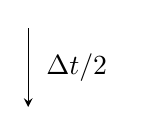
\begin{tikzpicture}[>=stealth]
                    \draw[->] (0,0) -- (0,-1) node[midway, right, xshift=3pt] {$\Delta t/2$};
                \end{tikzpicture}
            \end{center}
            \vspace{-0.2cm}
            \begin{minipage}{0.48\textwidth}
                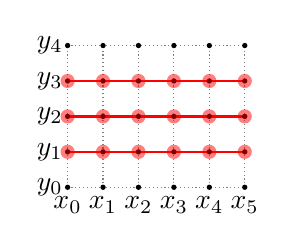
\begin{tikzpicture}[scale=0.45]
                    \foreach \y in {0,...,4} {
                         \draw[gray, densely dotted] (0,\y) -- (5,\y);
                         \node at (-0.5, \y) {$y_{\y}$};
                         \onslide<2->{
                         \ifnum \y = 1
                         \draw[red, thick] (0,1) -- (5,1);
                      \fi}
                        \onslide<3->{
                            \ifnum \y = 2
                            \draw[red, thick] (0,2) -- (5,2);
                            \fi
                        }
                        \onslide<4->{
                            \ifnum \y = 3
                            \draw[red, thick] (0,3) -- (5,3);
                            \fi
                        }
                     }
                                         
                     \foreach \x in {0,...,5} {
                         \draw[gray, densely dotted] (\x,0) -- (\x,4);
                         \node at (\x, -0.5) {$x_{\x}$};

                     }
                     \foreach \x in {0,...,5}
                         \foreach \y in {0,...,4} {
                             \fill (\x,\y) circle (0.0753); 
                             \onslide<2->{
                             \ifnum \y=1
                            \fill[red, fill opacity=0.5] (\x,\y) circle (0.2);
                            \fi
                            }
                            \onslide<3->{
                                \ifnum \y=2
                                \fill[red, fill opacity=0.5] (\x,\y) circle (0.2);
                                \fi
                            }
                            \onslide<4->{
                                \ifnum \y=3
                                \fill[red, fill opacity=0.5] (\x,\y) circle (0.2);
                                \fi
                            }
                         }
                \end{tikzpicture}
            \end{minipage}
            
        \end{column}
        \hspace{-0.8cm}
       \begin{column}{0.7\textwidth}
            %\footnotesize
            %we need smaller font size. let's try even smaller. Let's try tiny.
            \tiny
          \vspace{-1.5cm}  
          \onslide<2->{
                \begin{align*}
                    \begin{bmatrix}
                        1 + \alpha & -\alpha & 0 & 0 \\
                         -\alpha & 1 + 2\alpha & -\alpha & 0  \\
                        0 & -\alpha & 1 + 2\alpha & -\alpha \\
                         0 & 0 & -\alpha & 1 + \alpha \\
                    \end{bmatrix}
                    \begin{bmatrix}
                        \textcolor{red}{u_{1,1}^{k+\frac{1}{2}}} \\
                        \textcolor{red}{u_{2,1}^{k+\frac{1}{2}}} \\
                        \textcolor{red}{u_{3,1}^{k+\frac{1}{2}}} \\
                        \textcolor{red}{u_{4,1}^{k+\frac{1}{2}}} \\
                    \end{bmatrix}
                    =
                    \begin{bmatrix}
                        \textcolor{blue}{b_{1,1}} \\
                        \textcolor{blue}{b_{2,1}} \\
                        \textcolor{blue}{b_{3,1}} \\
                        \textcolor{blue}{b_{4,1}} \\
                    \end{bmatrix}
                \end{align*}
          }
                \vspace{-0.5cm}
                \onslide<3->{
                \begin{align*}
                    \begin{bmatrix}
                        1 + \alpha & -\alpha & 0 & 0  \\
                         -\alpha & 1 + 2\alpha & -\alpha & 0 \\
                        0 & -\alpha & 1 + 2\alpha & -\alpha \\
                         0 & 0 & -\alpha & 1 + \alpha  \\
                    \end{bmatrix}
                    \begin{bmatrix}
                        \textcolor{red}{u_{1,2}^{k+\frac{1}{2}}} \\
                        \textcolor{red}{u_{2,2}^{k+\frac{1}{2}}} \\
                        \textcolor{red}{u_{3,2}^{k+\frac{1}{2}}} \\
                        \textcolor{red}{u_{4,2}^{k+\frac{1}{2}}} \\
                    \end{bmatrix}
                    =
                    \begin{bmatrix}
                        \textcolor{blue}{b_{1,2}} \\
                        \textcolor{blue}{b_{2,2}} \\
                        \textcolor{blue}{b_{3,2}} \\
                        \textcolor{blue}{b_{4,2}} \\
                    \end{bmatrix}
                \end{align*}
                }
                \vspace{-0.5cm}
                \onslide<4->{
                \begin{align*}
                    \begin{bmatrix}
                        1 + \alpha & -\alpha & 0 & 0 \\
                         -\alpha & 1 + 2\alpha & -\alpha & 0  \\
                        0 & -\alpha & 1 + 2\alpha & -\alpha  \\
                         0 & 0 & -\alpha & 1 + \alpha  \\
                    \end{bmatrix}
                    \begin{bmatrix}
                        \textcolor{red}{u_{1,3}^{k+\frac{1}{2}}} \\
                        \textcolor{red}{u_{2,3}^{k+\frac{1}{2}}} \\
                        \textcolor{red}{u_{3,3}^{k+\frac{1}{2}}} \\
                        \textcolor{red}{u_{4,3}^{k+\frac{1}{2}}} \\
                    \end{bmatrix}
                    =
                    \begin{bmatrix}
                        \textcolor{blue}{b_{1,3}} \\
                        \textcolor{blue}{b_{2,3}} \\
                        \textcolor{blue}{b_{3,3}} \\
                        \textcolor{blue}{b_{4,3}} \\
                    \end{bmatrix}
                \end{align*}
                }
                \vspace{-1.5cm}
        \end{column}
    \end{columns}
   
    \vspace{0.1cm}
    \small
    \onslide<5->{
        Now we can use the Thomas algorithm for solving each tridiagonal system.
    }
\end{frame}


\end{document}